\documentclass[11pt,a4paper]{article}

\usepackage[a4paper, portrait, margin=1.1in]{geometry}
\usepackage[dvipsnames]{xcolor}
\usepackage[linktoc=none]{hyperref}
\hypersetup{
	colorlinks=true,
	linkcolor=blue,
	filecolor=magenta,      
	urlcolor=blue,
}

\usepackage{listings}
\usepackage{float}
\usepackage{graphicx}
\usepackage[justification=centering]{caption}
\usepackage{wrapfig}
\usepackage{amsmath}

\renewcommand{\contentsname}{Indice}

\definecolor{anti-flashwhite}{rgb}{0.95, 0.95, 0.96}

\begin{document}

\begin{center}
	\Large\textbf{Classificazione dei Supercomputer}\\
	\vspace{0.2cm}
	\large{Progetto per il corso di Statistica del Prof. Marco Romito}\\
	\vspace{0.5cm}
	\large\textit{Rambod Rahmani}\\
	\vspace{0.2cm}
	\scriptsize{Corso di Laurea Magistrale in\\Artificial Intelligence and
	Data Engineering}\\
	\vspace{0.5cm}
	\normalsize{13 Dicembre 2020}
\end{center}

\tableofcontents

\section{Introduzione}
Lo scopo della presente analisi \`e quello di costruire un modello di
regressione lineare multivariata per poter prevedere le prestazioni di un
Supercomputer a partire dalle specifiche delle sue caratteristiche hardware. A
partire dalla tabella dei dati, tramite l’utilizzo di R, sono stati valutati due
modelli diregressione. In particolare, uno di regressione lineare e uno di tipo
non lineare.\\
\\
Per quanto riguarda il contesto applicativo ipotizzato, esistono due benchmarks
essenziali che vengono usati per valutare le prestazioni di questo tipo di
calcolatori, il LINPACK benchmark (una misura delle prestazioni computazionali
per operazioni in virgola mobile) e il HPCG benchmark (a complemento del
LINPACK, valuta le prestazioni dei sotto sistemi del calcolatore). I costruttori
di tali computer forniscono di solito il parametro teorico (calcolato su carta)
chiamato \textbf{Rpeak} che indica le prestazioni massime teoriche. Dato che per
eseguire un test LINPACK \`e necessario calibrare ben oltre $18$ parametri,
sarebbe interessante poter stimare il valore di \textbf{Rmax} (prestazioni
raggiunte nel LINPACK test) tramite un modello statistico.

\section{Dati}
La tabella dei dati \`e stata scaricata dal sito dell'organizzazione
\textbf{TOP500}. La TOP500 mantiene una graduatoria, ordinata secondo le loro
prestazioni, dei Supercomputer attualmente installati e in funzione. Tale
graduatoria viene aggiornata con cadenza semestrale.\\
\textbf{Link di download diretto:} \url{https://www.top500.org/lists/top500/2020/11/download/TOP500_202011.xlsx}\\
\begin{figure}[h]
	\vspace{-1cm}
	\begin{minipage}{.3\textwidth}
		\textbf{Credenziali di accesso:}
	\end{minipage}
	\begin{minipage}{0.7\textwidth} 
		\begin{lstlisting}[language=bash,tabsize=2,backgroundcolor=\color{Goldenrod}]
		Login: rambodrahmani@yahoo.it
		Password: GCgFH6yuZYFMeCr
		\end{lstlisting}
	\end{minipage}
	\vspace{-1cm}
\end{figure}
\subsection{Contenuto della tabella}
La tabella dei dati contiene $37$ colonne per un totale di $500$ osservazioni.
Per la presente analisi ho utilizzato le seguenti colonne:
\begin{itemize}
	\setlength\itemsep{0mm}
	\item \textbf{Total Cores}: numero totale di cores;
	\item \textbf{Accelerator/Co-Processor Cores}: numero totale di
		cores del co-processore;
	\item \textbf{Rmax [TFlop/s]}: massime prestazioni raggiunte nel
		benchmark LINPACK;
	\item \textbf{Rpeak [TFlop/s]}: massime prestazioni teoriche;
	\item \textbf{HPCG [TFlop/s]}: massime prestazioni raggiunte nel
		benchmark HPCG (High Performance Conjugate Gradient);
	\item \textbf{Power [kW]}: potenza consumata;
	\item \textbf{Processor Speed [MHz]}: velocit\`a processore;
	\item \textbf{Cores per Socket}: numero di cores per socket.
\end{itemize}
\subsection{Importazione e pulizia}
Sui dati, non \`e stata effettuata alcuna operazione precedente la loro
importazione in R. Il file originale, in formato \texttt{.xlsx}, \`e stato
per\`o convertito in \texttt{.csv} per facilitare l'importazione.\\
Prima di iniziare l'analisi, ho rimosso le colonne che ritengo che non
influenzano le prestazioni di un Supercomputer ("Name", "Manufacturer",
"Country", "Year", ecc\dots), mentre come fattore di
uscita per la predizione utilizzer\`o il valore della colonna "Rmax".\\
Nelle colonne che ho scelto, ho rilevato $351$ valori mancanti in
"Accelerator/Co-Processor Cores", $426$ in "HPCG [TFlop/s]" e $310$ in
"Power [kW]". Dato che il numero di valori mancanti \`e elevato rispetto al
totale delle $500$ osservazioni, le suddette colonne sono state eliminate.
\begin{wrapfigure}{l}{1\textwidth}
	\vspace{-0.6cm}
	\centering
	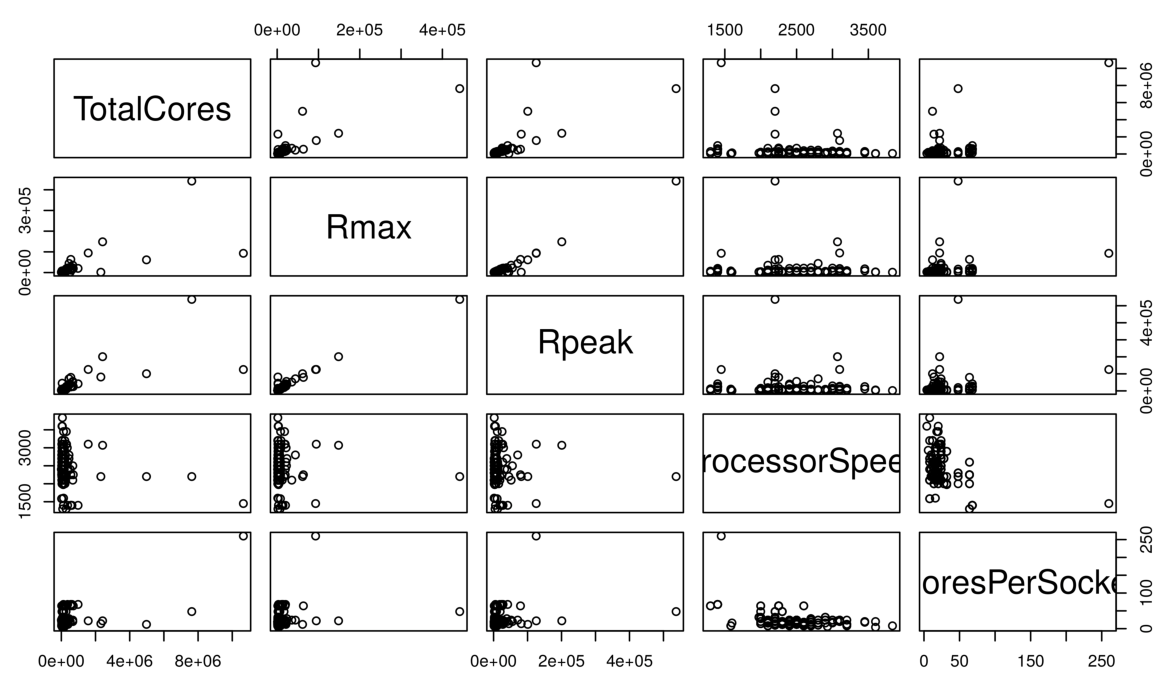
\includegraphics[scale=0.72]{imgs/plot(data).pdf}
	\vspace{-0.4cm}
	\caption{Diagramma di dispersione}
\end{wrapfigure}
\clearpage
\subsection{Esplorazione e comprensione dei dati}
\begin{wrapfigure}{r}{0.4\textwidth}
	\vspace{-1.3cm}
	\centering
	\caption{Matrice di dispersione}
	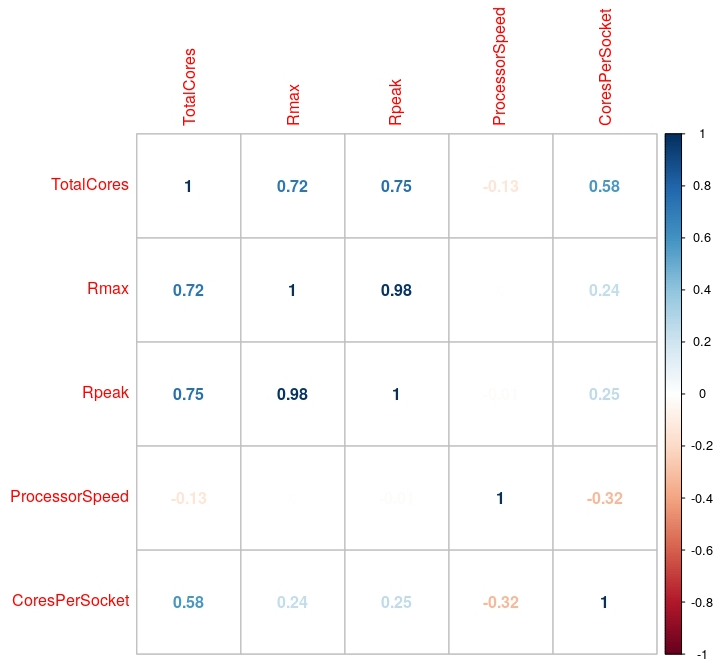
\includegraphics[scale=0.39]{imgs/cor_mat.jpeg}
	\vspace{-1.0cm}
\end{wrapfigure}
Il primo approcio esplorativo dei dati \`e stato di tipo grafico: nonostante si
possa palesemente vedere una forte correlazione tra il fattore di uscita
\textbf{Rmax} e i fattori \textbf{TotalCores} e \textbf{Rpeak}, ho preferito
iniziare con un modello di regressione lineare multipla usando \textbf{Rmax}
come output e tutte le altre variabili come predittori. Ho poi proceduto con
l'eliminazione dei fattori valutando per ogni modello ottenuto i seguenti
valori:
\begin{itemize}
	\setlength\itemsep{0mm}
	\item $\boldsymbol{R^2}$: Proporzione di Varianza Spiegata dal Modello;
	\item $\boldsymbol{R^2_{Adj}}$: Proporzione di Varianza Spiegata dal
		Modello corretto;
	\item \textbf{p-value} globale e dei singoli coefficienti.
\end{itemize}

\section{Analisi}
\subsection{Modello di Regressione Lineare}
Come primo passo, ho costruito $4$ differenti modelli di regressione lineare
valutando di volta in volta il valore di $\boldsymbol{R^2}$,
$\boldsymbol{R^2_{Adj}}$, \textbf{p-value}. Si pu\`o osservare un netto calo di
entrambi i grafici tra i punti di ascissa $3$ e $4$: dunque la terza versione
\`e la migliore delle quattro regressioni effettuate.
\begin{figure}[h]
	\hspace{-2.15cm}
	\begin{minipage}{.6\textwidth} 
		\begin{lstlisting}[language=bash,basicstyle=\tiny,tabsize=2,frame = single]
> summary(lm)

Call:
lm(formula = Rmax ~ Rpeak + TotalCores, data = data)

Residuals:
   Min     1Q Median     3Q    Max 
-59167    -74    478   1132  23307 

Coefficients:
              Estimate Std. Error t value Pr(>|t|)    
(Intercept) -1.101e+03  1.804e+02  -6.103 2.09e-09 ***
Rpeak        8.012e-01  9.450e-03  84.782  < 2e-16 ***
TotalCores  -1.392e-03  4.091e-04  -3.401 0.000724 ***
---
Signif. codes:  0 ‘***’ 0.001 ‘**’ 0.01 ‘*’ 0.05 ‘.’ 0.1 ‘ ’ 1

Residual standard error: 3889 on 497 degrees of freedom
Multiple R-squared:  0.9691,	Adjusted R-squared:  0.969 
F-statistic:  7800 on 2 and 497 DF,  p-value: < 2.2e-16
		\end{lstlisting}
	\end{minipage}
	\begin{minipage}{0.5\textwidth} 
		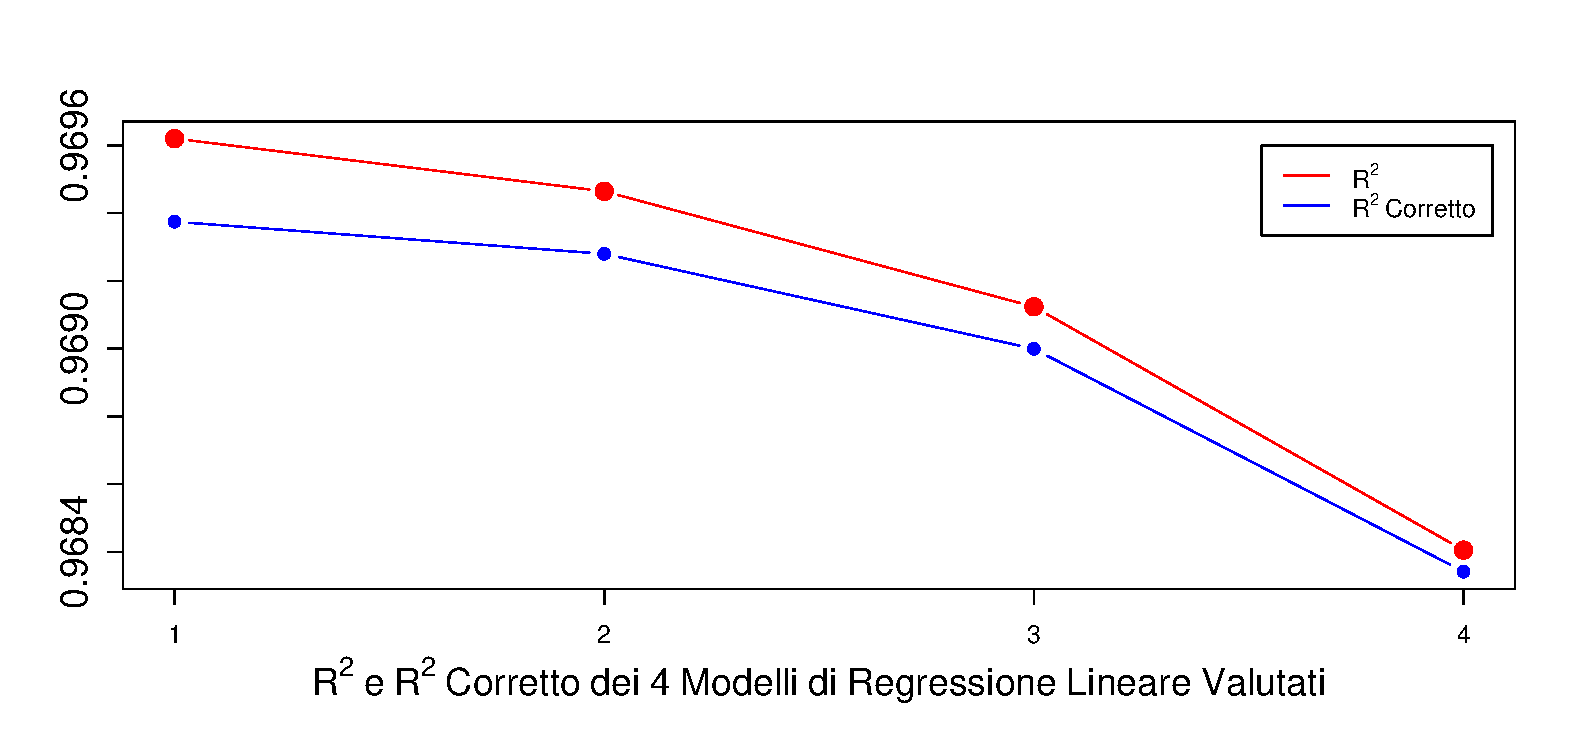
\includegraphics[scale=.4]{imgs/r_squared.pdf}
	\end{minipage}
\end{figure}
Con una proporzione di varianza spiegata dal modello maggiore del $96\%$ e con
dei p-value quasi nulli (sia per quanto riguarda i singoli coefficienti che
quello globale), possiamo concludere che il modello di regressione che abbiamo
ottenuto cattura buona parte del problema ed \`e statisticamente significativo.
\subsubsection{Analisi dei Residui}
Soddisfatto del modello ho proceduto con l'analisi dei residui. Dal diagramma di
dispersione, dall'istogramma, dal QQ\_plot, dal valore della skewness e della
kurtosi e dai risultati ottenuti dal Test di Shapiro-Wilk, \`e evidente che la
distribuzione dei residui \`e ben lontana dall'essere la Gaussiana che
cerchiamo:
\clearpage
\begin{figure}[H]
	\vspace{-1cm}
	\hspace{-1.5cm}
	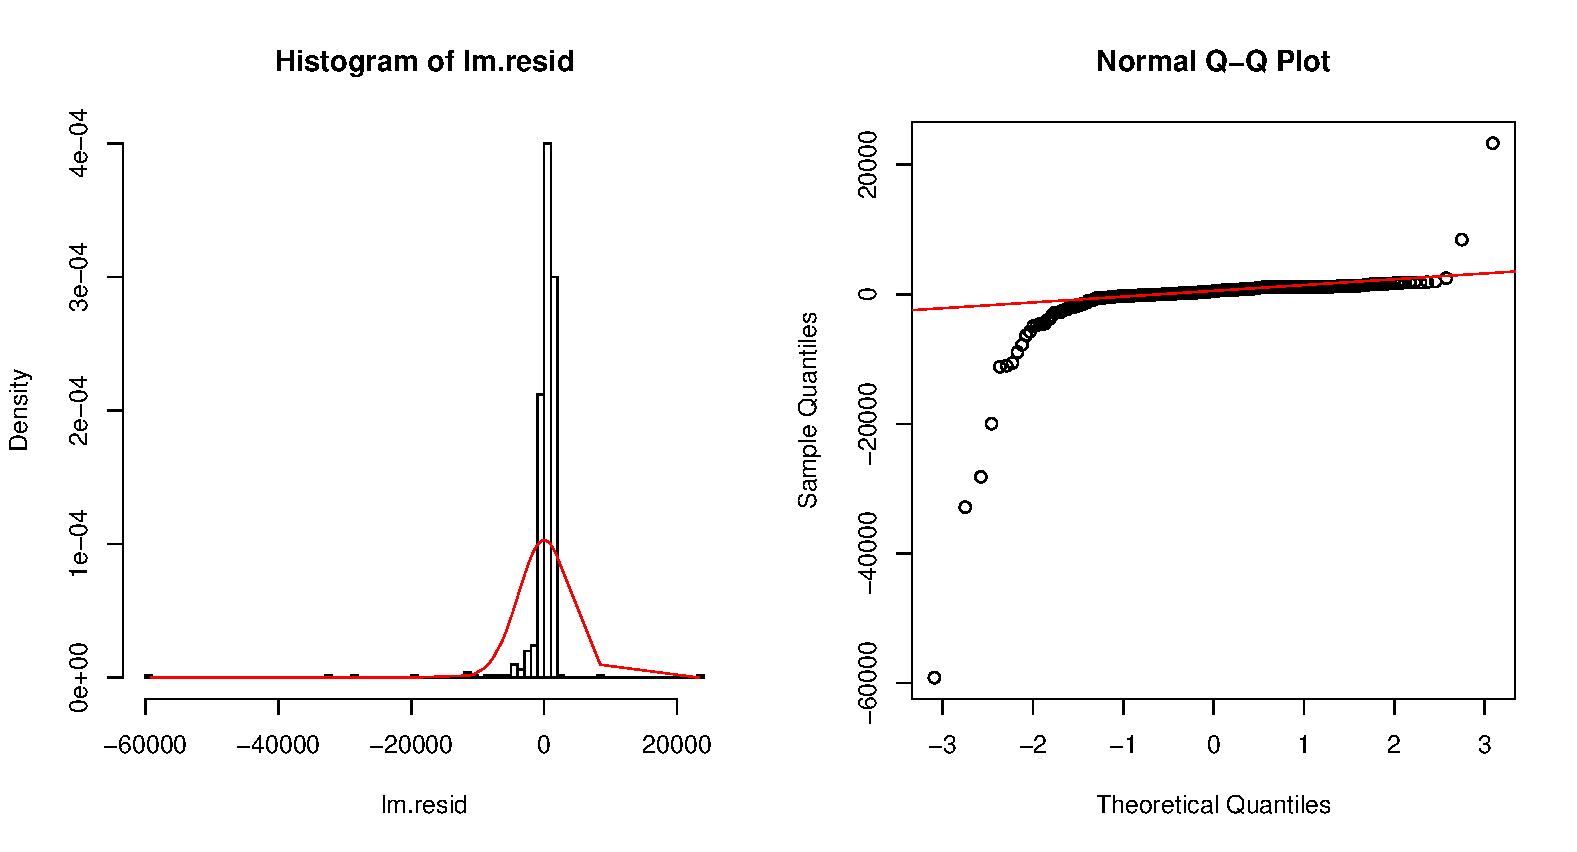
\includegraphics[scale=0.7]{imgs/residuals.pdf}
\end{figure}
\vspace{-0.8cm}
\begin{lstlisting}[language=bash,basicstyle=\tiny,tabsize=2,frame = single]
> skewness = mean(((lm.resid - mean(lm.resid)) / sd(lm.resid))^3); skewness
[1] -9.094902
> kurtosi = mean(((lm.resid - mean(lm.resid)) / sd(lm.resid))^4) - 3; kurtosi
[1] 125.4671

> shapiro.test(lm.resid)

	Shapiro-Wilk normality test

data:  lm.resid
W = 0.28981, p-value < 2.2e-16
\end{lstlisting}
\vspace{0.2cm}
Per approfondire, ho analizzato la correlazione tra i predittori utilizzati, se
eventualmente i residui del modello fossero correlati con uno dei predittori, un
modello di regressione con tutti i predittori disponibili e un modello di
regressione lineare semplice. I risultati per\`o non sono stati comunque
soddisfacenti:
\vspace{0.2cm}
\begin{lstlisting}[language=bash,basicstyle=\tiny,tabsize=2,frame = single]
> cor(data$Rpeak, data$TotalCores)
[1] 0.7525282
> cor(data$Rpeak, lm.resid)
[1] 1.965037e-15
> cor(data$TotalCores, lm.resid)
[1] 8.458876e-16

> # approfondimento analisi dei residui: valutazione modello di regressione lineare con tutti i fattori
> lm.1.resid = residuals(lm.1)
> shapiro.test(lm.1.resid)

	Shapiro-Wilk normality test

data:  lm.1.resid
W = 0.31715, p-value < 2.2e-16

> # approfondimento analisi dei residui: valutazione modello di regressione lineare semplice
> lm.4.resid = residuals(lm.4)
> shapiro.test(lm.4.resid)

	Shapiro-Wilk normality test

data:  lm.4.resid
W = 0.27671, p-value < 2.2e-16
\end{lstlisting}
\vspace{0.2cm}
La mia ipotesi allora, dato che la distribuzione \`e comunque centrata in zero e
ricorda l'andamento di una Gaussiana, e dato il valore di kurtosi pari a
$125.4671$ \`e stata che fosse a causa della presenza di alcuni valori numerici
eccessivamente elevati rispetto alla media. Dopo aver rimosso questo primo
sottoinsieme di residui, ho notato che probabilmente fosse necessario rimuovere
una parte dei residui che causavano una forte deviazione da una distribuzione
Gaussiana. Cos\`i facendo ho ottenuto un modello certamente migliore ma
comunque non perfetto:
\clearpage
\begin{figure}[H]
	\vspace{-1.5cm}
	\begin{center}
		\hspace*{-1.5cm}
		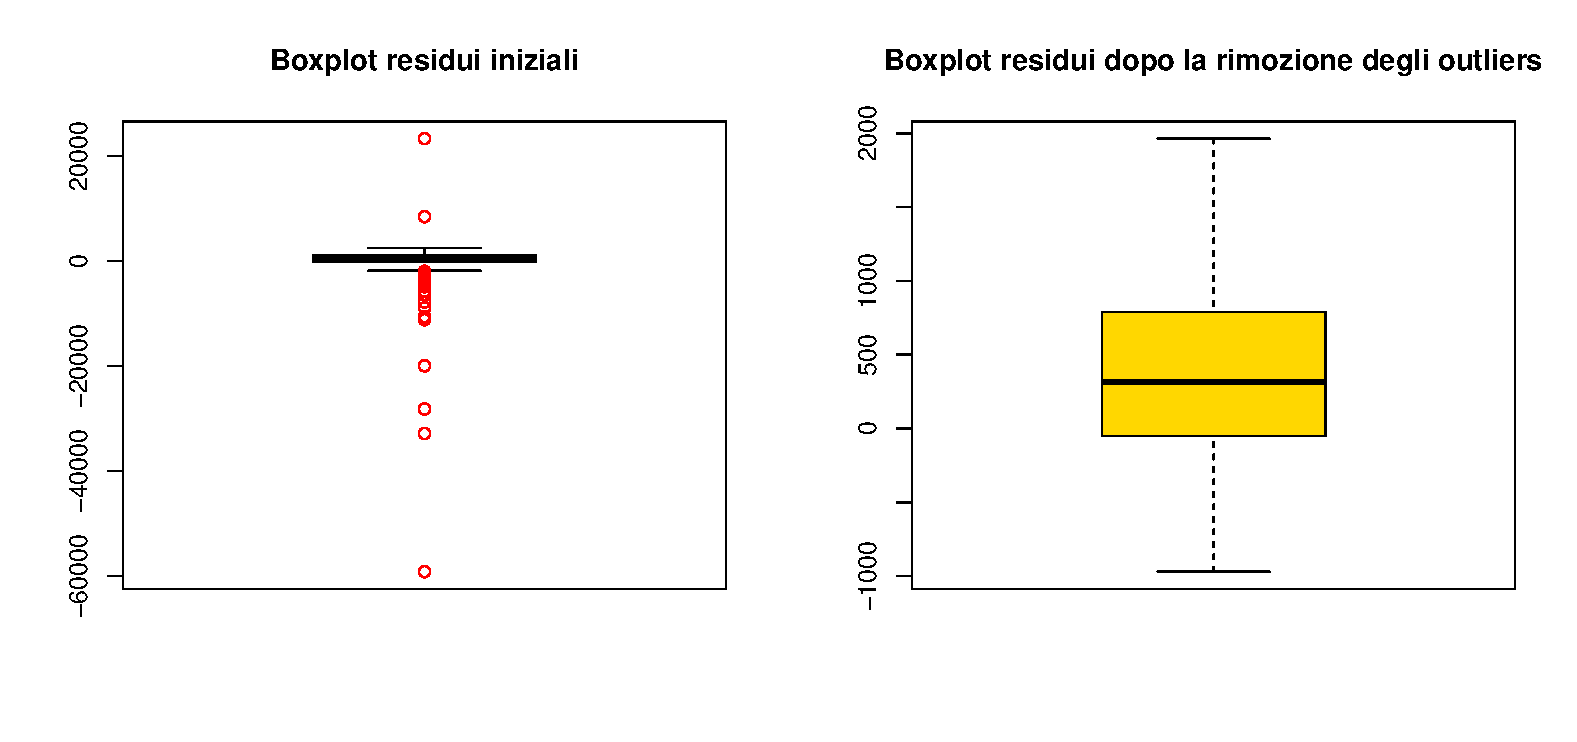
\includegraphics[scale=0.7]{imgs/residuals_boxplots.pdf}
	\end{center}
\end{figure}
\vspace{-2.2cm}\noindent
Per la precisione, sono stati rimossi $40$ campioni per ottenere il seguente
risultato:
\vspace{-0.1cm}
\begin{figure}[H]
	\begin{center}
		\hspace*{-1.5cm}
		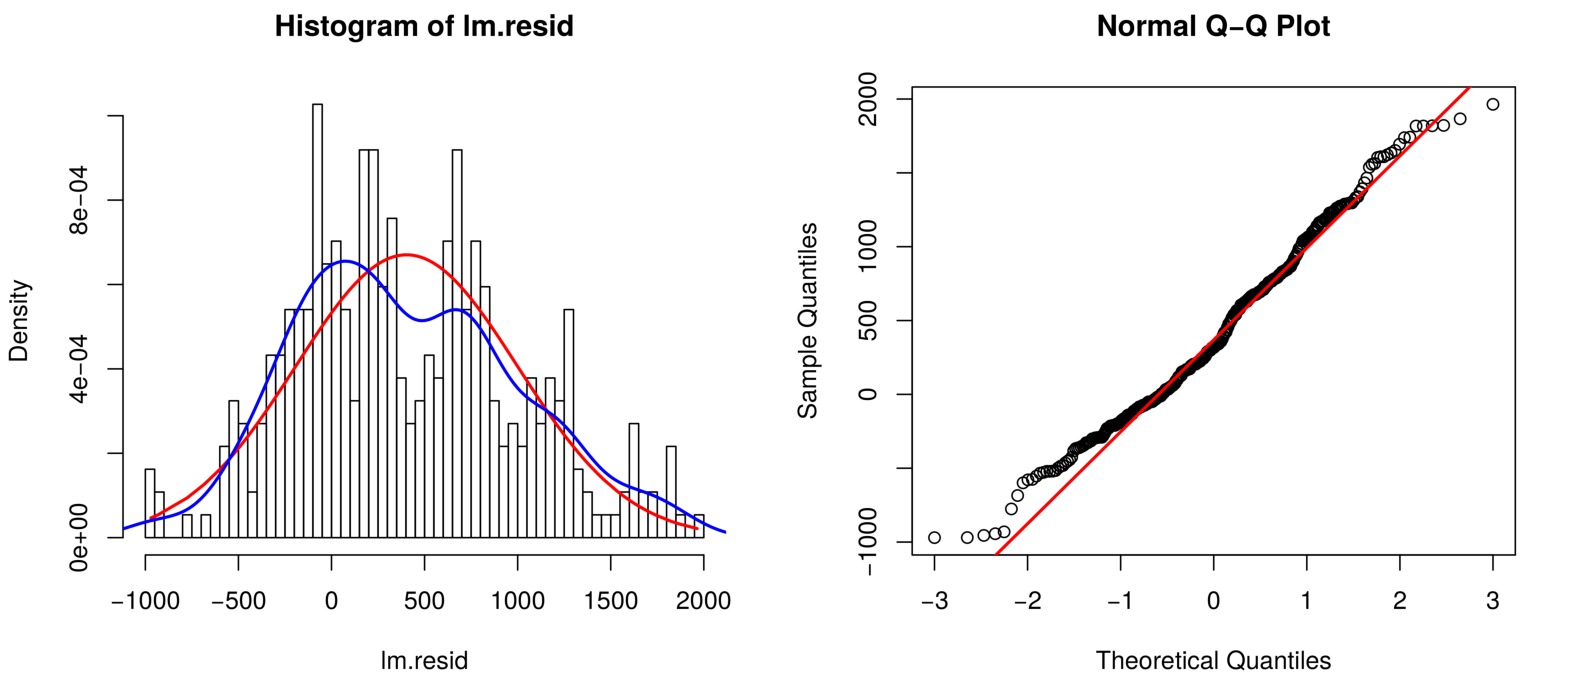
\includegraphics[scale=0.7]{imgs/residuals_2.pdf}
	\end{center}
\end{figure}
\vspace{-1.1cm}
\begin{lstlisting}[language=bash,basicstyle=\tiny,tabsize=2,frame = single]
> skewness = mean(((lm.resid - mean(lm.resid)) / sd(lm.resid))^3); skewness
[1] 0.2961855

> kurtosi = mean(((lm.resid - mean(lm.resid)) / sd(lm.resid))^4) - 3; kurtosi
[1] -0.3962842

> shapiro.test(lm.resid)

	Shapiro-Wilk normality test

data:  lm.resid
W = 0.98522, p-value = 0.0007833
\end{lstlisting}
Da notare comunque la diminuzione del valore del p-value di ben oltre $10$
ordini di grandezza nel Test di Shapiro-Wilk, e il netto miglioramento dei
valori di skewness e kurtosi. Dobbiamo certamente sottolineare che, con una
proporzione di varianza spiegata dal modello pari al $96\%$, l'errore introdotto
dalla non normalit\`a della distribuzione dei residui, rappresenta una
piccolissima parte di struttura che non riusciamo a catturare.
\subsection{Modello di Regressione Logaritmico}
Non contento, nella speranza di riuscire ad ottenere un modello di regressione
con un valore di $\boldsymbol{R^2}$ leggermente minore, ma con una distribuzione
dei residui migliore, ho provato una analisi tramite modello di regressione non
lineare. Quindi ho usato la trasformazione logaritmica per effettuare un
\textit{fit} esponenziale. Seguendo lo stesso filone di ragionamento e con le
dovute accortezze, riassumo di seguito i risultati ottenuti:
\clearpage
\begin{figure}[h]
	\vspace{-1.5cm}
	\hspace{-2.15cm}
	\begin{minipage}{.6\textwidth} 
		\begin{lstlisting}[language=bash,basicstyle=\tiny,tabsize=2,frame = single]
> summary(lm)

Call:
lm(formula = log(Rmax) ~ log(Rpeak) + log(TotalCores), data = data)

Residuals:
     Min       1Q   Median       3Q      Max 
-3.12824 -0.08284  0.07566  0.12253  0.88843 

Coefficients:
                Estimate Std. Error t value Pr(>|t|)    
(Intercept)     -0.24672    0.19428  -1.270    0.205    
log(Rpeak)       0.65997    0.02967  22.246  < 2e-16 ***
log(TotalCores)  0.23030    0.02847   8.088 4.66e-15 ***
---
Signif. codes:  0 ‘***’ 0.001 ‘**’ 0.01 ‘*’ 0.05 ‘.’ 0.1 ‘ ’ 1

Residual standard error: 0.3061 on 497 degrees of freedom
Multiple R-squared:  0.8203,	Adjusted R-squared:  0.8195 
F-statistic:  1134 on 2 and 497 DF,  p-value: < 2.2e-16
		\end{lstlisting}
	\end{minipage}
	\begin{minipage}{0.5\textwidth} 
		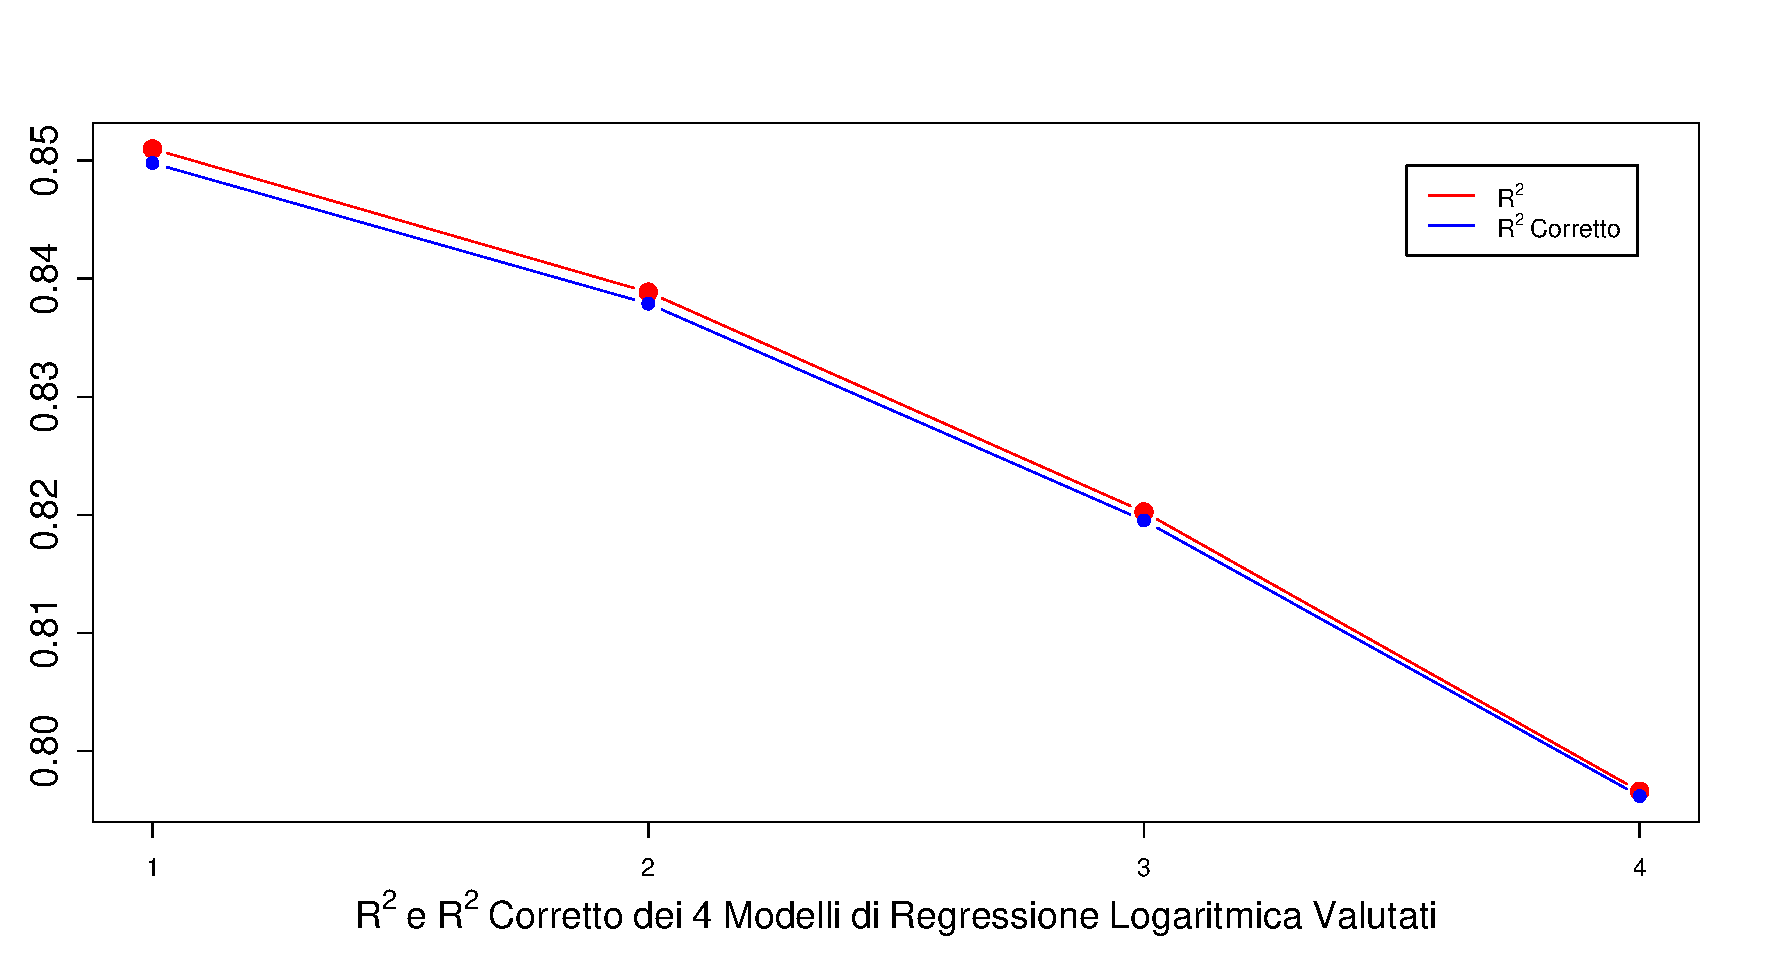
\includegraphics[scale=.36]{imgs/r_squared_log.pdf}
	\end{minipage}
\end{figure}
\vspace{-0.4cm}\noindent
Notiamo quindi un passaggio da una Varianza spiegata del $96\%$ con un modello
di regressione lineare, all'$82\%$ del modello logaritmico.
\subsubsection{Analisi dei Residui}
I valori di partenza dell'analisi dei residui riguardanti il modello
logaritmico non sono certamente perfetti ma comunque migliori di quelli del
modello lineare.
\begin{figure}[H]
	\hspace{-1.5cm}
	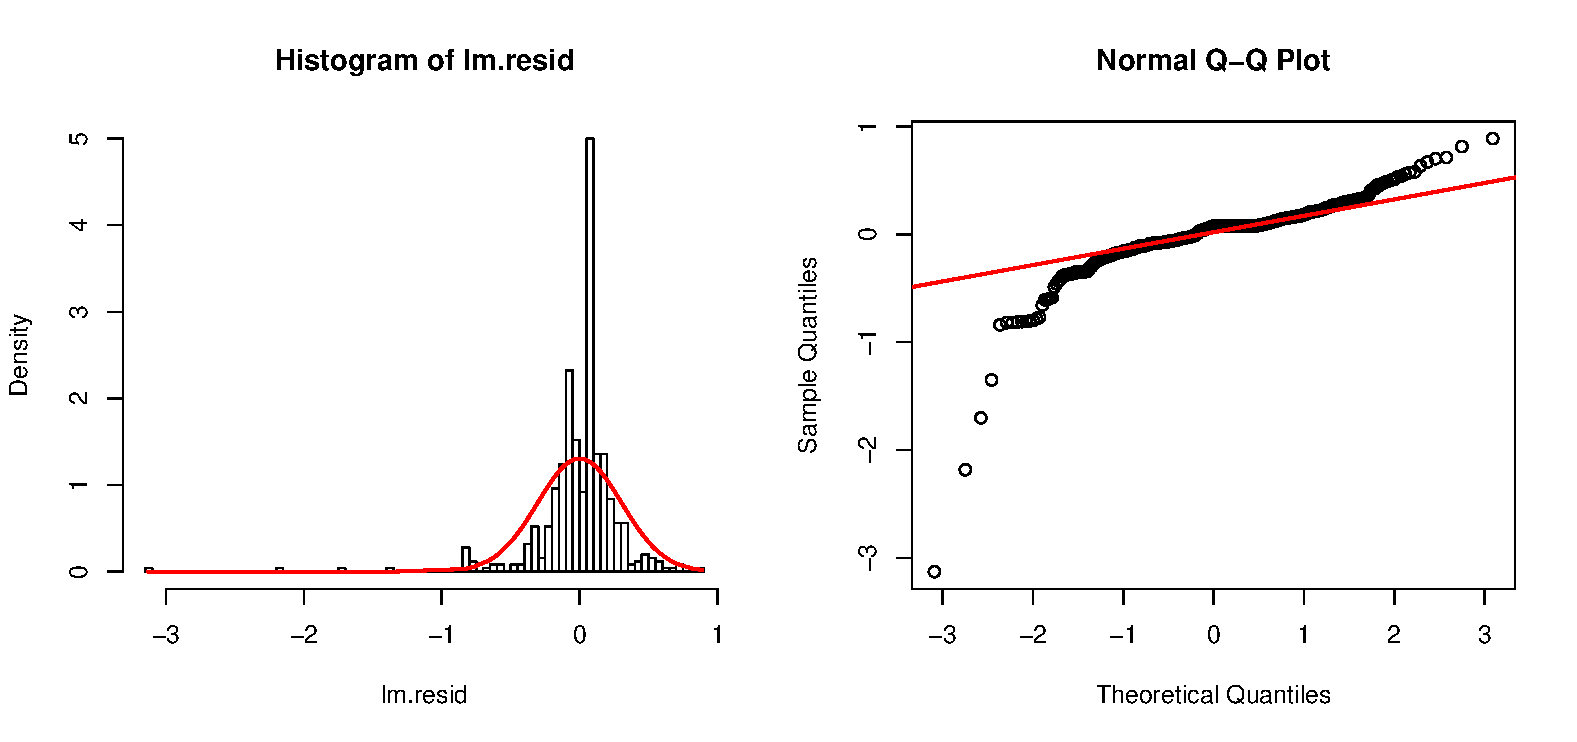
\includegraphics[scale=0.7]{imgs/residuals_log.pdf}
\end{figure}
\vspace{-0.8cm}
\begin{lstlisting}[language=bash,basicstyle=\tiny,tabsize=2,frame = single]
> skewness = mean(((lm.resid - mean(lm.resid)) / sd(lm.resid))^3); skewness
[1] -3.561324

> kurtosi = mean(((lm.resid - mean(lm.resid)) / sd(lm.resid))^4) - 3; kurtosi
[1] 28.8915

> shapiro.test(lm.resid)

	Shapiro-Wilk normality test

data:  lm.resid
W = 0.74598, p-value < 2.2e-16
\end{lstlisting}
Ugualmente a quanto fatto nell'analisi dei residui del modello di regressione
lineare, ho rimosso una parte dei residui che causavano una forte deviazione da
una distribuzione Gaussiana. \textbf{La presenza di questi residui "anomali", in
entrambi i modelli valutati, \`e dovuta alla presenza di osservazioni "anomale"
che dipendono dal fatto che la tabella di dati raccoglie informazioni
riguardanti Supercomputer dal 2010 al 2020. Sappiamo bene quanto aumentino
bruscamente le prestazioni dei computer in un arco di tempo pari a 10 anni. In
questo contesto quindi, per "anomalo" non intendiamo certo errato ma bens\`i
diverso. L'analisi di regressione sicuramente soffre per la presenza di questi
fattori.}
\begin{figure}[H]
	\vspace{-1.3cm}
	\begin{center}
		\hspace*{-1.5cm}
		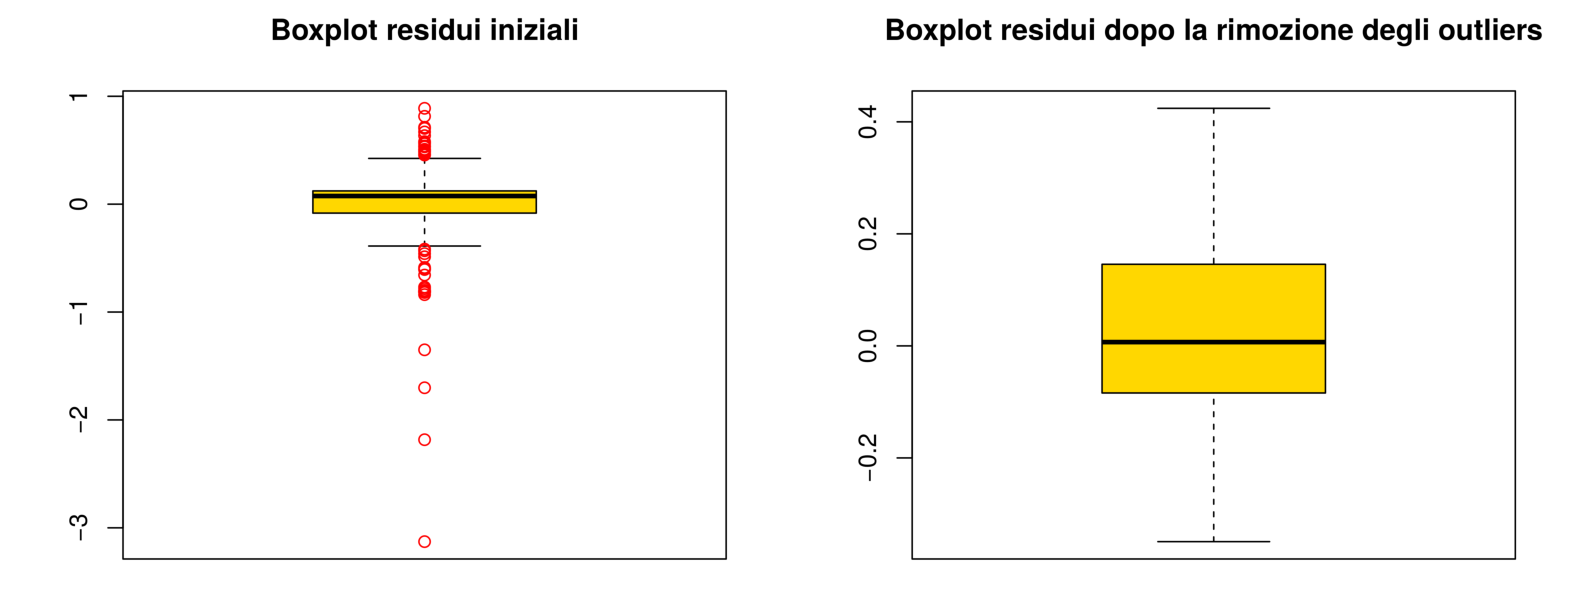
\includegraphics[scale=0.7]{imgs/residuals_boxplots_log.pdf}
	\end{center}
\end{figure}
\vspace{-1cm}\noindent
Per la precisione, sono stati rimossi $40$ campioni per ottenere il seguente
risultato:
\begin{figure}[H]
	\begin{center}
		\hspace*{-1.5cm}
		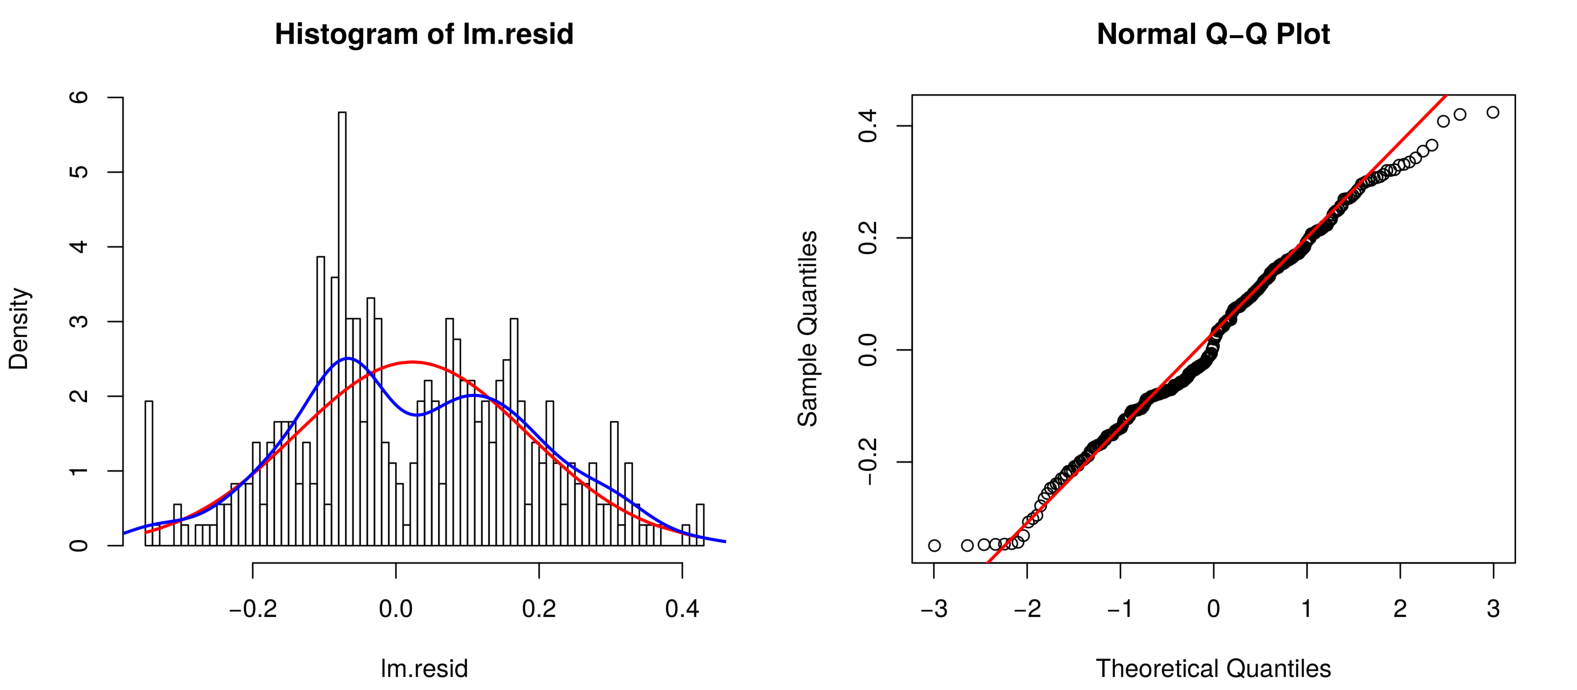
\includegraphics[scale=0.7]{imgs/residuals_2_log.pdf}
	\end{center}
\end{figure}
\vspace{-0.9cm}
\begin{lstlisting}[language=bash,basicstyle=\tiny,tabsize=2,frame = single]
> skewness = mean(((lm.resid - mean(lm.resid)) / sd(lm.resid))^3); skewness
[1] 0.04635719

> kurtosi = mean(((lm.resid - mean(lm.resid)) / sd(lm.resid))^4) - 3; kurtosi
[1] -0.5150052

> shapiro.test(lm.resid)

	Shapiro-Wilk normality test

data:  lm.resid
W = 0.98905, p-value = 0.008154
\end{lstlisting}
I valori di skewness e kurtosi sono certamente accetabili anche se il
\textbf{p-value} del Test di Shapiro-Wilk, che comunque \`e \textbf{migliorato
aumentando di un ordine di grandezza} rispetto ai residui del modello di
regressione lineare, rimane comunque ancora basso. Dobbiamo infatti tenere a
mente che questo miglioramento dei risultati del Test di Shapiro-Wilk lo stiamo
pagando in termini del valore di $\boldsymbol{R^2}$ che \`e passato, lo
ricordiamo, da $96\%$ a $82\%$. A questo punto, per esprimere un giudizio finale
definitivo, comparer\`o i due modelli in fase di predizione.
\section{Predizione e autovalutazione}
Dato che, al termine del processo di eliminazione dei fattori, ho ottenuto un
modello, sia nel caso lineare che nel caso logaritmico, con due predittori e un
fattore di uscita, ho pensato di rappresentare entrambi i modelli tramite una
grafico di dispersione 3D:
\begin{figure}[H]
	\begin{center}
		\hspace*{-2.7cm}
		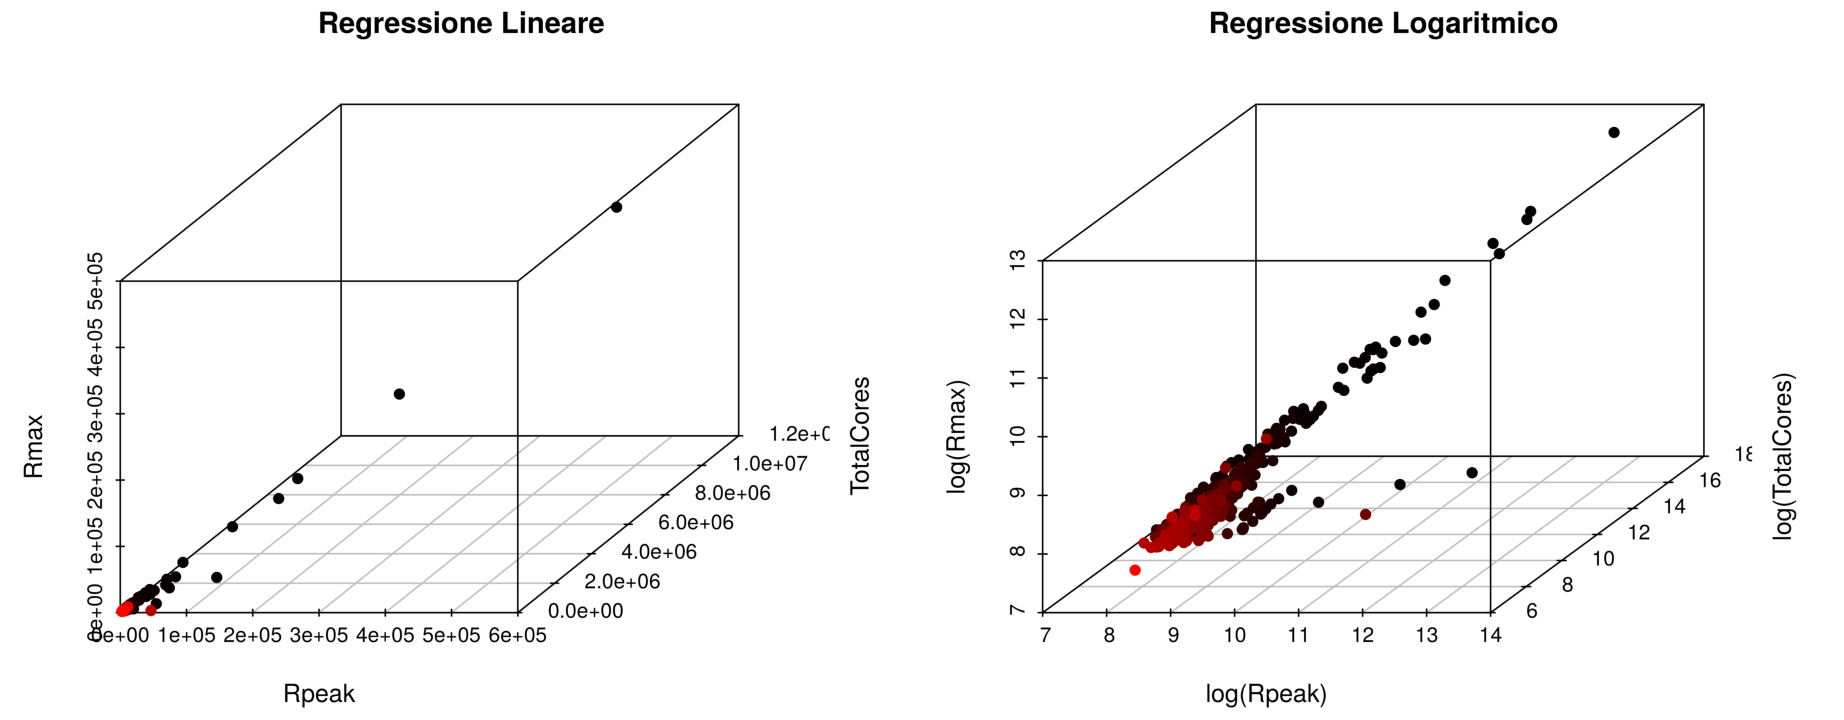
\includegraphics[scale=0.66]{imgs/scatterplot_3d.pdf}
		\vspace{-1cm}
	\end{center}
\end{figure}
\noindent
Ritengo che sia utile dato che ci mostra in maniera visiva quanto abbiamo
concluso nelle fasi precedenti della nostra analisi: il modello logaritmico,
tramite il cambio di scala, riesce ad attenuare l'affetto dispersivo dovuto
alla presenza degli outliers nella tabella di dati originale.\\
\\
In fase di predizione e autovalutazione, i due modelli sono stati messi a
confronto. Le osservazioni della tabella originale sono state suddivise in un
sottoinsieme di $50$ osservazioni, utilizzato come insieme di predizione, e un
sottoinsieme di $450$ osservazioni, utilizzato come insieme di allenamento del
modello. Ho osservato che questa diminuzione del numero di osservazioni
utilizzato per la costruzione dei due modelli non ha inciso drasticamente sulla
proporzione di varianza spiegata dal modello. Oscilla intorno al $96\%$ per
quanto riguarda il modello libeare e intorno al $82\%$ per quanto riguarda il
modello logaritmico.
\begin{lstlisting}[language=bash,basicstyle=\tiny,tabsize=2,frame = single]
> summary(data_train.lm)$r.squared
[1] 0.9692249

> summary(ldata_train.lm)$r.squared
[1] 0.8195792

> data_train.lm.p = predict(data_train.lm, data_test)
> ldata_train.lm.p = predict(ldata_train.lm, ldata_test)

> sqrt(mean((data_train.lm.p - data_train$Rmax)^2))
[1] 23126.91

> sqrt(mean((exp(ldata_train.lm.p) - data_train$Rmax)^2))
[1] 23190.9
\end{lstlisting}
Considerare lo scarto medio di una sola estrazione di sottoinsiemi, di un solo
esperimento quindi, non porta certamente risultati statisticamente
significativi. Ho ripetuto l'esperimento quindi $50$ volte:
\begin{lstlisting}[language=bash,basicstyle=\tiny,tabsize=2,frame = single]
> mean(err_lin)
[1] 24802.19

> mean(err_log)
[1] 22593.09

> sd(err_lin)
[1] 6244.185

> sd(err_log)
[1] 782.1269
\end{lstlisting}
In media quindi, il modello logaritmico, ha una media di errore pi\`u bassa.
Inoltre, la deviazione standard del modello logaritmico \`e nettamente
inferiore rispetto a quella del modello
\clearpage
\vspace*{-1.5cm}
\noindent
lineare, possiamo quindi considerarlo molto pi\`u affidabile. La seguente figura
riassume la simulazione eseguita:
\begin{figure}[H]
	\begin{center}
		\vspace{-0.4cm}
		\hspace*{-2.7cm}
		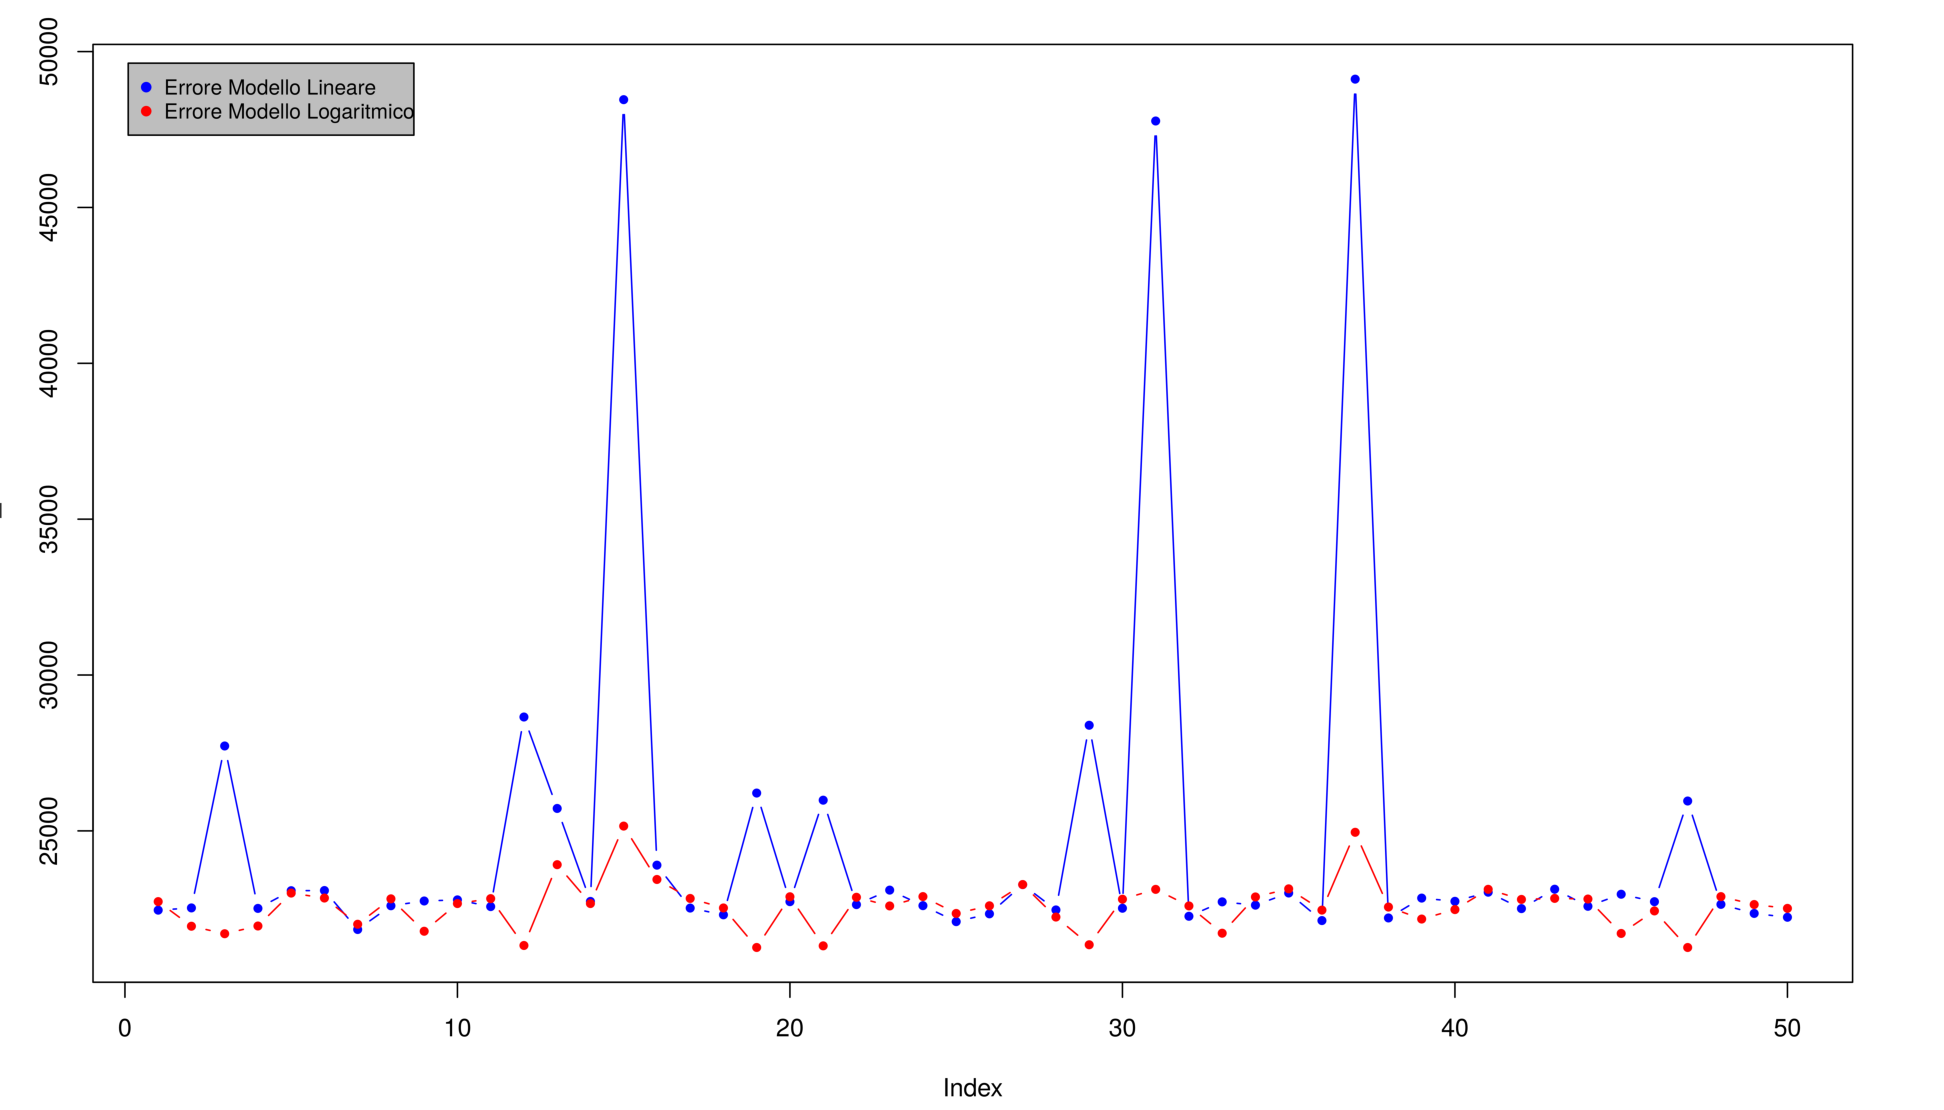
\includegraphics[scale=0.65]{imgs/simulation.pdf}
		\vspace{-1.5cm}
	\end{center}
\end{figure}
\section{Conclusioni}
In ultima analisi, la mia ipotesi, utilizzare un modello non lineare con la
trasformazione logaritmica, perdendo qualcosa in Varianza Spiegata dal
modello per ottenere un andamento dei residui pi\`u "normale", si \`e rivelata
corretta. Quando ho terminato la messa a punto dei due modelli, mi era difficile
valutare tramite i vari diagrammi e i valori numerici dei test eseguiti. In fase
di predizione e autovalutazione i miei dubbi sono stati risolti dai risultati
della simulazione: effettivamente, il modello logaritmico in media sbaglia di
meno, e ha un comportamento, in fase di predizione, pi\`u affidabile rispetto al
modello lineare.\\
Bisogna tenere in considerazione anche il fatto che la tabella presenta un
numero consistente di fattori qualitativi che non abbiamo preso in
considerazione, dato che ci siamo basati esclusivamente sui fattori
quantitativi. Tali fattori, forse, potrebbero aiutarci a ottenere un
$\boldsymbol{R^2}$ pi\`u elevato per il modello logaritmico e residui
migliori.\\
\\
Per quanto riguarda le considerazioni relative al contesto applicativo della
presente analisi, sulle quali non mi sono voluto dilungare nella sezione
introduttiva per lasciare spazio all'analisi stessa, certamente un modello
statistico di questo tipo, che permetta di predire il valore \textbf{Rmax} per
un Supercomputer, \`e utile in quanto:
\begin{itemize}
	\setlength\itemsep{0mm}
	\item il "high-performance LINPACK (HPL) benchmark" richiede la
		calibrazione di ben oltre $18$ parametri per essere eseguito;
	\item un errore nella calibrazione di uno solo di questi parametri pu\`o
		compromettere (eventualmente falsare) i risultati ottenuti;
	\item mantenere un Supercomputer acceso per l'esecuzione dell'HPL ha un
		consumo enegetico non indifferente.
\end{itemize}
\end{document}
